% ========================================
% FRAMEWORK AT A GLANCE
% Minimalist one-page cheat sheet inserted after TOC, before Foreword
% ========================================

\thispagestyle{empty}  % No page number
\begin{center}

\vspace*{0.5cm}

{\LARGE\textbf{Framework at a Glance}}

\vspace{0.5cm}

% ========================================
% I. THE SORT FRAMEWORK (4 Fundamental Axes)
% ========================================

{\large\textbf{I. The SORT Framework}}
\vspace{0.2cm}

\begin{small}
\begin{tabular}{@{}llll@{}}
\toprule
\textbf{Axis} & \textbf{Question} & \textbf{-1 Pole} & \textbf{+1 Pole} \\
\midrule
\textbf{S} (Sovereignty) & Who are we? & Individual & Collective \\
\textbf{O} (Organization) & How do we build? & Emergence & Design \\
\textbf{R} (Reality) & How do we know? & Mythos & Gnosis \\
\textbf{T} (Telos) & What do we seek? & Homeostasis & Metamorphosis \\
\bottomrule
\end{tabular}
\end{small}

\vspace{0.4cm}

% ========================================
% II. THE PHASE SPACE DIAGRAMS (Master Dynamics)
% ========================================

{\large\textbf{II. The Phase Space (Master Dynamics)}}
\vspace{0.2cm}

% Two diagrams side by side
\begin{minipage}[t]{0.48\textwidth}
\centering
{\small\textbf{Α-Ω (Pedagogical Simplification)}}
\vspace{0.1cm}

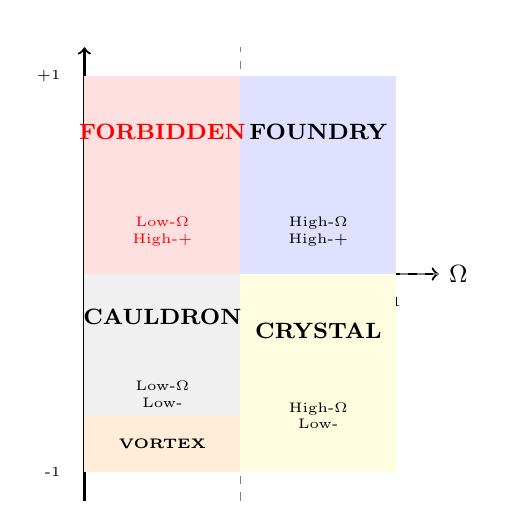
\begin{tikzpicture}[scale=1.8]
    % Axes
    \draw[->,thick] (0,0) -- (2.5,0) node[right,font=\small] {$\Omega$};
    \draw[->,thick] (0,-1.6) -- (0,1.6) node[above,font=\small] {$\Alpha$};

    % Ticks
    \node[below,font=\tiny] at (2.2,-0.1) {1};
    \node[left,font=\tiny] at (-0.1,1.4) {+1};
    \node[left,font=\tiny] at (-0.1,-1.4) {-1};

    % Quadrant boundaries
    \draw[gray,thin,dashed] (1.1,-1.6) -- (1.1,1.6);
    \draw[gray,thin,dashed] (0,0) -- (2.5,0);

    % Quadrant fills and labels (SMALLER TEXT)
    \fill[blue!12] (1.1,0) rectangle (2.2,1.4);
    \node[align=center,font=\footnotesize\bfseries] at (1.65, 1.0) {FOUNDRY};
    \node[align=center,font=\tiny] at (1.65, 0.3) {High-$\Omega$\\High-$\Alpha$+};

    \fill[red!12] (0,0) rectangle (1.1,1.4);
    \node[align=center,font=\footnotesize\bfseries,red] at (0.55, 1.0) {FORBIDDEN};
    \node[align=center,font=\tiny,red] at (0.55, 0.3) {Low-$\Omega$\\High-$\Alpha$+};

    \fill[yellow!12] (1.1,-1.4) rectangle (2.2,0);
    \node[align=center,font=\footnotesize\bfseries] at (1.65, -0.4) {CRYSTAL};
    \node[align=center,font=\tiny] at (1.65, -1.0) {High-$\Omega$\\Low-$\Alpha$};

    \fill[gray!12] (0,-1.4) rectangle (1.1,0);
    \node[align=center,font=\footnotesize\bfseries] at (0.55, -0.3) {CAULDRON};
    \node[align=center,font=\tiny] at (0.55, -0.85) {Low-$\Omega$\\Low-$\Alpha$};

    % Vortex sub-region
    \fill[orange!15] (0,-1.4) rectangle (1.1,-1.0);
    \node[align=center,font=\tiny\bfseries] at (0.55, -1.2) {VORTEX};
\end{tikzpicture}
\end{minipage}
\hfill
\begin{minipage}[t]{0.48\textwidth}
\centering
{\small\textbf{T-Ω (Causal Mechanics)}}
\vspace{0.1cm}

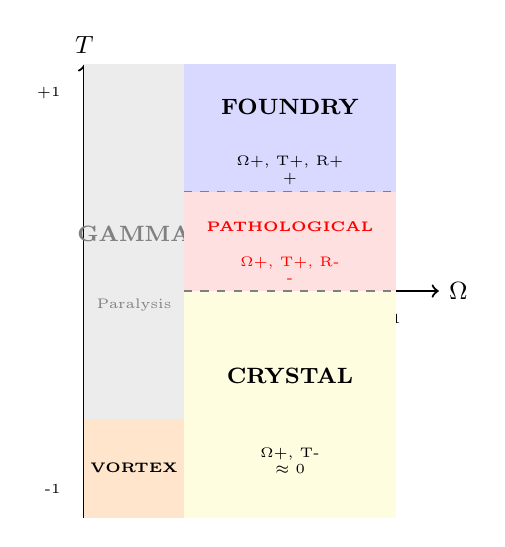
\begin{tikzpicture}[scale=1.8]
    % Axes
    \draw[->,thick] (0,0) -- (2.5,0) node[right,font=\small] {$\Omega$};
    \draw[->,thick] (0,-1.6) -- (0,1.6) node[above,font=\small] {$T$};

    % Ticks
    \node[below,font=\tiny] at (2.2,-0.1) {1};
    \node[left,font=\tiny] at (-0.1,1.4) {+1};
    \node[left,font=\tiny] at (-0.1,-1.4) {-1};

    % Iron Law threshold
    \draw[red,thick,dashed] (0.7,-1.6) -- (0.7,1.6);
    \node[red,font=\tiny,align=center,rotate=90] at (0.4,0) {Iron Law};

    % LEFT REGION: Low-Ω
    \fill[gray!15] (0,-1.6) rectangle (0.7,1.6);
    \node[align=center,font=\footnotesize\bfseries,gray] at (0.35,0.4) {GAMMA};
    \node[align=center,font=\tiny,gray] at (0.35,-0.1) {Paralysis};

    \fill[orange!20] (0,-1.6) rectangle (0.7,-0.9);
    \node[align=center,font=\tiny\bfseries] at (0.35,-1.25) {VORTEX};

    % Bottom-Right: High-Ω, T-
    \fill[yellow!12] (0.7,-1.6) rectangle (2.2,0);
    \node[align=center,font=\footnotesize\bfseries] at (1.45,-0.6) {CRYSTAL};
    \node[align=center,font=\tiny] at (1.45,-1.2) {$\Omega$+, T-\\$\Alpha \approx 0$};

    % Top-Right: Foundry (R+ upper, R- lower)
    \fill[blue!15] (0.7,0.7) rectangle (2.2,1.6);
    \node[align=center,font=\footnotesize\bfseries] at (1.45,1.3) {FOUNDRY};
    \node[align=center,font=\tiny] at (1.45,0.85) {$\Omega$+, T+, R+\\$\Alpha$+};

    \fill[red!12] (0.7,0) rectangle (2.2,0.7);
    \node[align=center,font=\tiny\bfseries,red] at (1.45,0.45) {PATHOLOGICAL};
    \node[align=center,font=\tiny,red] at (1.45,0.15) {$\Omega$+, T+, R-\\$\Alpha$-};

    % Divider
    \draw[gray,thin,dashed] (0.7,0) -- (2.2,0);
    \draw[gray,thin,dashed] (0.7,0.7) -- (2.2,0.7);
\end{tikzpicture}
\end{minipage}

\vspace{0.3cm}

\begin{small}
\textbf{$\Omega$ (Coherence):} Internal unity (0 = fragmented, 1 = unified) \quad
\textbf{$\Alpha$ (Action):} Net output (-1 = entropic, +1 = syntropic)

\textbf{Iron Law of Coherence (Theorem):} Low-Ω, High-Α+ is \textit{impossible}. Synergy is non-negotiable precondition for Syntropy. The Α-Ω diagram shows \textit{observed outputs}; T-Ω reveals \textit{causal mechanics}.
\end{small}

\vspace{0.4cm}

% ========================================
% III. THE FOUR VIRTUES (IFHS)
% ========================================

{\large\bfseries III. The Four Virtues (The Optimal Solution)}
\vspace{0.3cm}

\begin{small}
\begin{tabular}{@{} >{\bfseries}l >{\itshape}l p{9cm} @{}}
\toprule
Virtue & Solves & Definition \\
\midrule
Integrity (I) & R-Axis & The Gnostic pursuit of a truthful Mythos (Truth + Meaning). \\
\addlinespace
Fecundity (F) & T-Axis & The creation of stable conditions for new growth (Stability + Growth). \\
\addlinespace
Harmony (H) & O-Axis & The use of minimal Design to unleash maximal Emergence (Order + Freedom). \\
\addlinespace
Synergy (S) & S-Axis & An architecture where the whole is greater than the sum of its parts (Individual + Collective = superadditive value). \\
\bottomrule
\end{tabular}
\end{small}

\vspace{0.6cm}

% ========================================
% IV. THE 3-LAYER ARCHITECTURE
% ========================================

{\large\bfseries IV. The 3-Layer Architecture (The Engineered Form)}
\vspace{0.3cm}

\begin{small}
\begin{tabular}{@{} >{\bfseries}l >{\itshape}l p{8cm} @{}}
\toprule
Layer & Function & Core Axiological Mode \\
\midrule
Head & Direction (T+) & \textbf{Instrumental:} Gnostic, Metamorphic, Pragmatic \\
\addlinespace
Skeleton & Constraint (T-) & \textbf{Protocol:} Gnostic, Designed, Principled \\
\addlinespace
Heart & Continuity (T-) & \textbf{Integrative:} Mythopoetic, Emergent, Somatic \\
\bottomrule
\end{tabular}
\end{small}

\vspace{0.3cm}
\begin{small}
\textit{Holographic Principle: This scale-invariant architecture is the stable solution for cells, organisms, individuals, and civilizations.}
\end{small}

\end{center}

\cleardoublepage
